\documentclass[12pt]{article}

\usepackage{sbc-template}
\usepackage{graphicx,url}
\usepackage[brazil]{babel}
\usepackage[utf8]{inputenc}
\usepackage[T1]{fontenc}
\usepackage{enumitem}
\usepackage{placeins}
\usepackage{booktabs}

\graphicspath{{figuras/}}

\setlength{\textfloatsep}{5pt plus 2pt minus 2pt}
\setlength{\intextsep}{5pt plus 2pt minus 2pt}
\setlength{\floatsep}{5pt plus 2pt minus 2pt}
\setlength{\abovecaptionskip}{3pt}

\sloppy

\title{Avaliação de Branch Prediction em RISC-V com o simulador gem5:\\
LocalBP versus BiModeBP e a sensibilidade ao padrão da carga}

\author{João Luís Almeida Santos\inst{1}}

\address{Bacharelado em Ciência da Computação\\
  Organização de Computadores (ORG 2026.1)
  \email{joao.santos@abensoft.com.br}
}

\begin{document}

\maketitle

\begin{abstract}
  This work evaluates the impact of two conditional branch predictors,
  LocalBP (a simple local predictor) and BiModeBP (a complex global
  predictor), on a branch-heavy RISC-V workload: a Monte Carlo RPG combat
  engine running 1{,}000 automated matches per workload. The assembly code from the
  first assignment was ported to the GCC syntax, compiled to a static
  RISC-V binary and simulated on gem5 with an out-of-order CPU. We extract
  and compare misprediction rate, IPC, total simulated time and squashed
  instructions from the generated \texttt{stats.txt}. BiModeBP reduced the
  conditional misprediction rate from 11.27\% to 8.57\%, raised IPC by
  3.8\% and cut wasted speculative work by 38\%.
\end{abstract}

\begin{resumo}
  Este trabalho avalia o impacto de dois preditores de desvios
  condicionais, LocalBP (preditor local simples) e BiModeBP (preditor
  global complexo), sobre uma carga de trabalho com forte presença de
  desvios: um motor de combate de RPG por Monte Carlo que simula
  1.000 partidas. O código \emph{assembly} do primeiro trabalho foi
  adaptado para a sintaxe do GCC, compilado em um binário estático
  RISC-V e simulado no gem5 com uma CPU fora de ordem. Extraímos e
  comparamos a taxa de erro de predição, o IPC, o tempo total de
  simulação e as instruções descartadas do \texttt{stats.txt} gerado.
  O BiModeBP reduziu a taxa de erro de 11,27\% para 8,57\%, elevou o
  IPC em 3,8\% e diminuiu em 38\% o trabalho especulativo desperdiçado.
\end{resumo}

\section{Introdução}

Preditores de desvio são componentes centrais de microarquiteturas
modernas: em um pipeline profundo, cada desvio condicional mal previsto
força o descarte (\emph{squash}) de todas as instruções buscadas
especulativamente após ele, pagando uma penalidade de vários ciclos
\cite{hennessy2017quantitative}. O ganho de um bom preditor depende
diretamente do padrão de desvios da carga de trabalho.

A carga avaliada é o algoritmo desenvolvido no Trabalho~1: um motor de
combate de RPG escrito inteiramente em RISC-V que executa uma simulação
Monte Carlo de 1.000 partidas entre três estratégias de IA distintas.
Como cada turno é decidido por máquinas de estado e por números
pseudoaleatórios (XORShift de Marsaglia~\cite{marsaglia2003xorshift}), o
código é dominado por desvios condicionais dependentes de dados --- o
cenário ideal para estressar um preditor.

Seguindo o Tópico~2 da proposta (\emph{Branch Prediction}), comparamos
dois extremos de preditor condicional do gem5~\cite{binkert2011gem5}: o
\textbf{LocalBP} (local simples) e o \textbf{BiModeBP} (global complexo).
As métricas exigidas --- desvios avaliados e erros de predição --- saem do
\texttt{stats.txt} de cada execução, complementadas por IPC, tempo de
simulação e instruções descartadas.

\section{Fundamentação Teórica}

\subsection{LocalBP --- preditor local}

O \textbf{LocalBP} mantém uma tabela de contadores saturados de 2 bits
indexada pelo PC do desvio; cada entrada guarda o histórico de
tomadas/não-tomadas \emph{daquele} desvio individualmente
\cite{smith1981branch}. É simples e barato, mas ignora correlação entre
desvios distintos e sofre \emph{aliasing} destrutivo quando vários desvios
disputam a mesma entrada.

\subsection{BiModeBP --- preditor global bimodal}

O \textbf{BiModeBP}~\cite{lee1997bimode} combina o histórico \emph{global}
recente com o PC para indexar duas tabelas de predição --- uma ``tomada''
e outra ``não tomada'' --- mais uma tabela de escolha. Ao separar os
desvios por sua tendência predominante, reduz a interferência destrutiva
entre desvios opostos e captura correlações globais, ao custo de mais área
e complexidade.

\section{Metodologia}

\subsection{Adaptação do código e compilação}

O \emph{assembly} original (\texttt{main.s}) foi escrito para o ambiente
RARS, que oferece \emph{syscalls} simplificadas e ponto de entrada
próprio. Para o gem5 foi produzida a versão \texttt{main\_gem5.s},
ajustando diretivas e o ponto de entrada \texttt{\_start} para a sintaxe
do GCC. O binário estático foi gerado com:

\begin{quote}\small\ttfamily
riscv64-linux-gnu-gcc -nostdlib -static main\_gem5.s -o output/main\_gem5
\end{quote}

A \emph{flag} \texttt{-static} produz o binário autocontido exigido pelo
modo \emph{Syscall Emulation} (SE) do gem5 e \texttt{-nostdlib} dispensa a
\emph{libc}. O artefato \texttt{output/main\_gem5} é o binário simulado em
ambos os cenários.

\subsection{Configuração do gem5}

O \emph{script} de configuração (\texttt{models/inorder.py}) monta uma
\texttt{SimpleBoard} a 1\,GHz com hierarquia de cache privada
L1 (32\,kB I + 32\,kB D) e L2 de 256\,kB, e memória DDR3-1600 de 1\,GB.
Apenas o preditor condicional é trocado entre as execuções:

\begin{quote}\small\ttfamily
processor.cores[0].core.branchPred.conditionalBranchPred = LocalBP()\\
\# ou BiModeBP()
\end{quote}

As duas simulações foram disparadas via \texttt{make run-bp}, gravando
resultados em \texttt{m5out/local/} e \texttt{m5out/bimode/}.

\noindent\textbf{Modelo de CPU.} O MinorCPU (\emph{In-Order} detalhado)
sofre um \emph{crash} conhecido na versão 25.1 do gem5 para RISC-V em modo
SE (\emph{bug} no \texttt{ActivityRecorder}); por isso ambos os cenários
usam o \texttt{DerivO3CPU}. Como o \emph{único} parâmetro alterado entre as
execuções é o preditor, a comparação isola o efeito da predição de desvios
e ainda permite medir o trabalho especulativo descartado (Tópico~4).

\noindent\textbf{Determinismo.} A \emph{seed} pseudoaleatória deriva do
tempo de execução, logo os contadores absolutos diferem um pouco entre as
execuções; a análise privilegia \emph{taxas e razões} (taxa de erro, IPC),
robustas a essa variação.

\subsection{Duas cargas de trabalho}
\label{sec:cargas}

Como um preditor só ganha explorando \emph{regularidade}, variamos o quão
previsível é a carga --- atendendo também ao pedido de ``diferentes cargas
de trabalho''. O motor de combate possui três bots: \emph{Flowey} (RNG
puro, sorteia a habilidade 1--6), \emph{Chara} (combo determinístico) e
\emph{Toby} (contra-estratégia). Avaliamos duas cargas:

\begin{itemize}[nosep]
  \item \textbf{Mista} (\texttt{main\_gem5.s}): a estratégia de cada
    jogador é sorteada por partida --- mistura de bots determinísticos e
    aleatórios, parcialmente estruturada.
  \item \textbf{Aleatória} (\texttt{main\_gem5\_random.s}): ambos os
    jogadores são fixados em \emph{Flowey}, de modo que toda decisão de
    habilidade é um sorteio uniforme. A variante foi \emph{clonada} do
    original alterando apenas a atribuição de estratégia no \texttt{\_start},
    sem tocar no binário base.
\end{itemize}

\noindent Cada carga foi simulada com os dois preditores (4 execuções,
1.000 partidas cada).

\section{Resultados}

A Tabela~\ref{tab:metricas} reúne as métricas extraídas do
\texttt{stats.txt} de cada cenário. A taxa de erro de predição é
calculada como \texttt{condIncorrect / condPredicted}.

\begin{table}[ht]
\centering
\caption{Métricas extraídas do \texttt{stats.txt} (gem5, DerivO3CPU).}
\label{tab:metricas}
\begin{tabular}{lrr}
\toprule
\textbf{Métrica} & \textbf{LocalBP} & \textbf{BiModeBP} \\
\midrule
Desvios cond. avaliados (\texttt{condPredicted}) & 900.700 & 803.703 \\
Desvios cond. incorretos (\texttt{condIncorrect}) & 101.531 & 68.838 \\
\textbf{Taxa de erro de predição} & \textbf{11,27\%} & \textbf{8,57\%} \\
IPC (\texttt{ipc}) & 1,4603 & 1,5165 \\
Tempo simulado (\texttt{simSeconds}) & 7,539\,ms & 7,181\,ms \\
Ciclos (\texttt{numCycles}) & 7.538.818 & 7.180.697 \\
Instruções efetivadas (\texttt{commit.numInsts}) & 11.009.088 & 10.889.293 \\
Instruções descartadas (\texttt{squashedInstsIssued}) & 102.245 & 62.953 \\
Acertos de BTB (\texttt{BTBHits}/\texttt{BTBLookups}) & 71,9\% & 70,9\% \\
\bottomrule
\end{tabular}
\end{table}

\subsection{Erros de predição}

A Figura~\ref{fig:mispred} mostra a métrica central do Tópico~2. O
BiModeBP errou em 8,57\% dos desvios condicionais contra 11,27\% do
LocalBP --- uma redução relativa de \textbf{24\%} na taxa de erro. A
Figura~\ref{fig:branches} contextualiza: ainda que o número absoluto de
desvios avaliados varie entre as execuções (efeito da \emph{seed}), a
fração de erros cai claramente com o preditor global.

\begin{figure}[ht]
\centering
\begin{minipage}{0.48\textwidth}
  \centering
  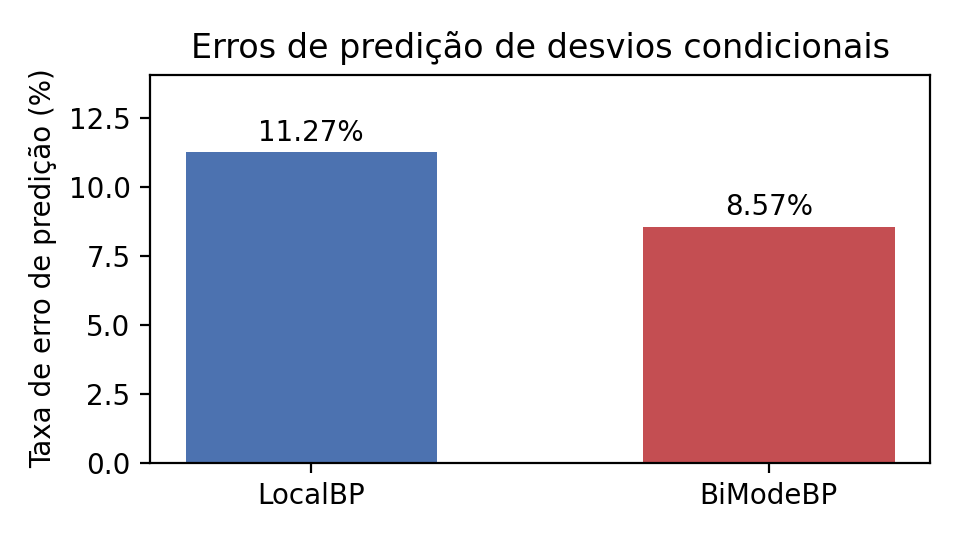
\includegraphics[width=\textwidth]{mispred.png}
  \caption{Taxa de erro de predição de desvios condicionais.}
  \label{fig:mispred}
\end{minipage}\hfill
\begin{minipage}{0.48\textwidth}
  \centering
  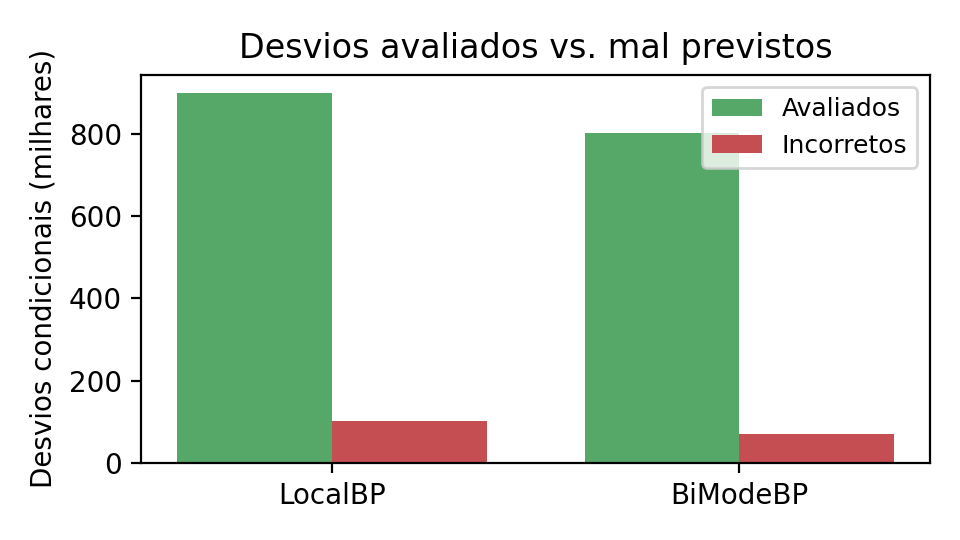
\includegraphics[width=\textwidth]{branches.png}
  \caption{Desvios avaliados vs. mal previstos.}
  \label{fig:branches}
\end{minipage}
\end{figure}

\subsection{Impacto no desempenho}

Menos erros de predição significam menos descartes e melhor
aproveitamento do pipeline. O IPC subiu de 1,4603 para 1,5165 (\textbf{+3,8\%}, Fig.~\ref{fig:ipc}) e
o tempo de simulação caiu 4,7\% (Fig.~\ref{fig:simtime}). O efeito mais
marcante está na Figura~\ref{fig:squashed}: o BiModeBP descartou 62,9\,mil
instruções especulativas contra 102,2\,mil do LocalBP --- \textbf{38\%}
menos trabalho desperdiçado.

\begin{figure}[ht]
\centering
\begin{minipage}{0.32\textwidth}
  \centering
  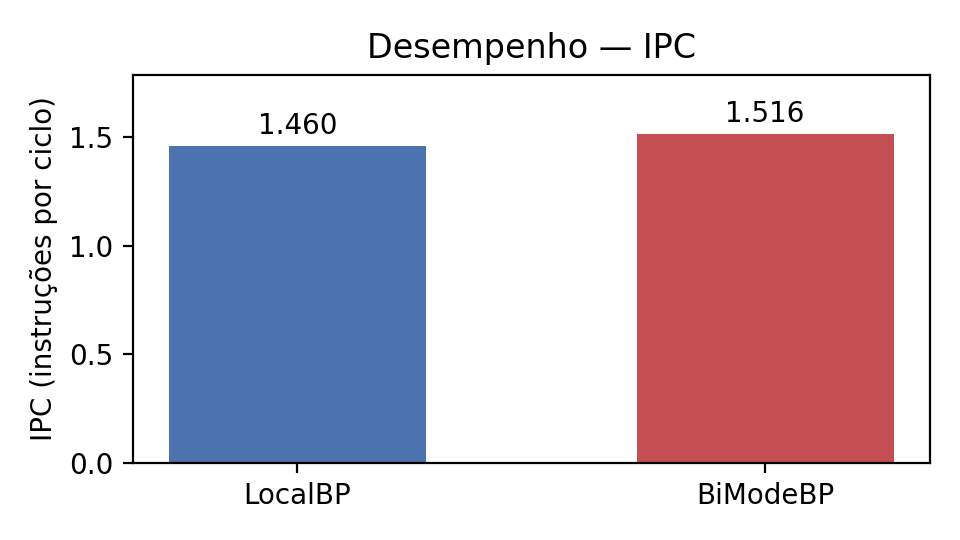
\includegraphics[width=\textwidth]{ipc.png}
  \caption{IPC.}
  \label{fig:ipc}
\end{minipage}\hfill
\begin{minipage}{0.32\textwidth}
  \centering
  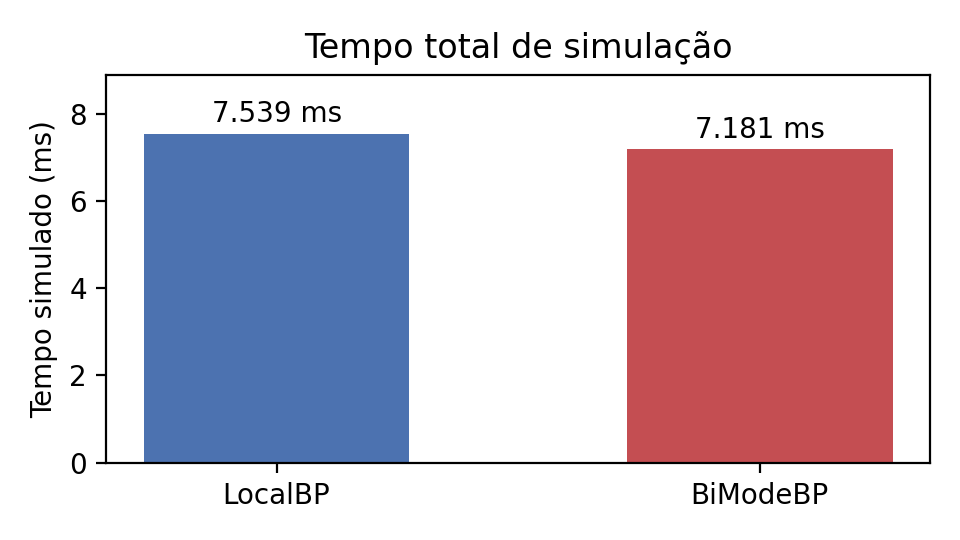
\includegraphics[width=\textwidth]{simtime.png}
  \caption{Tempo de simulação.}
  \label{fig:simtime}
\end{minipage}\hfill
\begin{minipage}{0.32\textwidth}
  \centering
  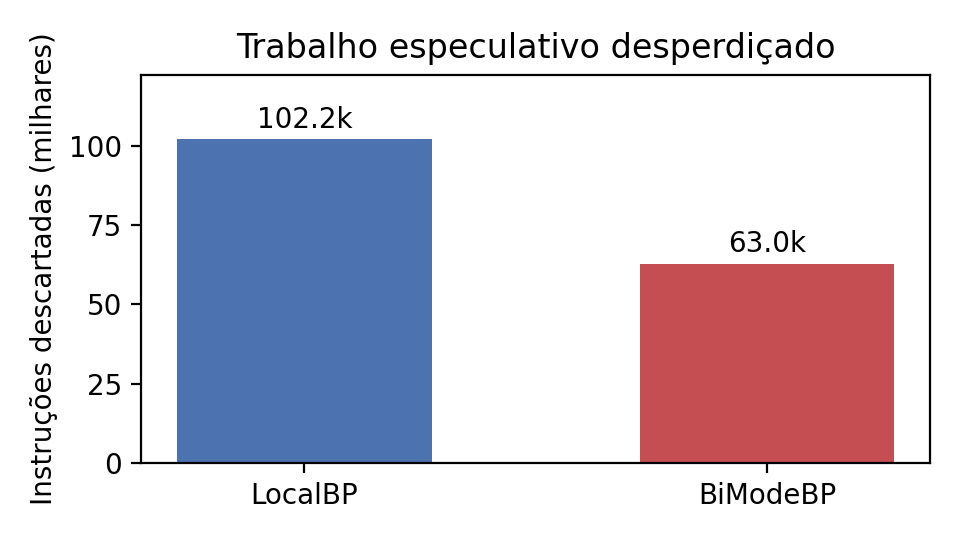
\includegraphics[width=\textwidth]{squashed.png}
  \caption{Descartadas.}
  \label{fig:squashed}
\end{minipage}
\end{figure}

\FloatBarrier

\subsection{Sensibilidade ao padrão de desvios da carga}
\label{sec:sensibilidade}

A Tabela~\ref{tab:cargas} repete o experimento na carga \emph{aleatória}
(Seção~\ref{sec:cargas}). Dois efeitos aparecem. Primeiro, \textbf{ambos}
os preditores pioram: a taxa de erro do LocalBP sobe de 11,27\% para
12,59\% e a do BiModeBP de 8,57\% para 10,07\%, pois a escolha uniforme de
habilidade transforma parte dos desvios em moedas justas, que nenhum
histórico prevê. Segundo, e mais revelador, \textbf{a vantagem do BiModeBP
encolhe}: de 24\% para 20\% de redução relativa do erro
(Figura~\ref{fig:wladv}). Quanto mais aleatória a carga, menor o retorno do
preditor sofisticado --- seu ganho vem justamente da estrutura que a
aleatoriedade destrói.

\begin{table}[ht]
\centering
\caption{Carga mista vs. aleatória, por preditor.}
\label{tab:cargas}
\small
\begin{tabular}{lrrrr}
\toprule
 & \multicolumn{2}{c}{\textbf{Mista}} & \multicolumn{2}{c}{\textbf{Aleatória}} \\
\cmidrule(lr){2-3}\cmidrule(lr){4-5}
\textbf{Métrica} & Local & BiMode & Local & BiMode \\
\midrule
Taxa de erro & 11,27\% & 8,57\% & 12,59\% & 10,07\% \\
IPC & 1,460 & 1,517 & 1,418 & 1,480 \\
Descartadas (mil) & 102,2 & 62,9 & 167,0 & 126,5 \\
Vantagem BiMode & \multicolumn{2}{c}{$-24\%$ erro} & \multicolumn{2}{c}{$-20\%$ erro} \\
\bottomrule
\end{tabular}
\end{table}

\begin{figure}[ht]
\centering
\begin{minipage}{0.48\textwidth}
  \centering
  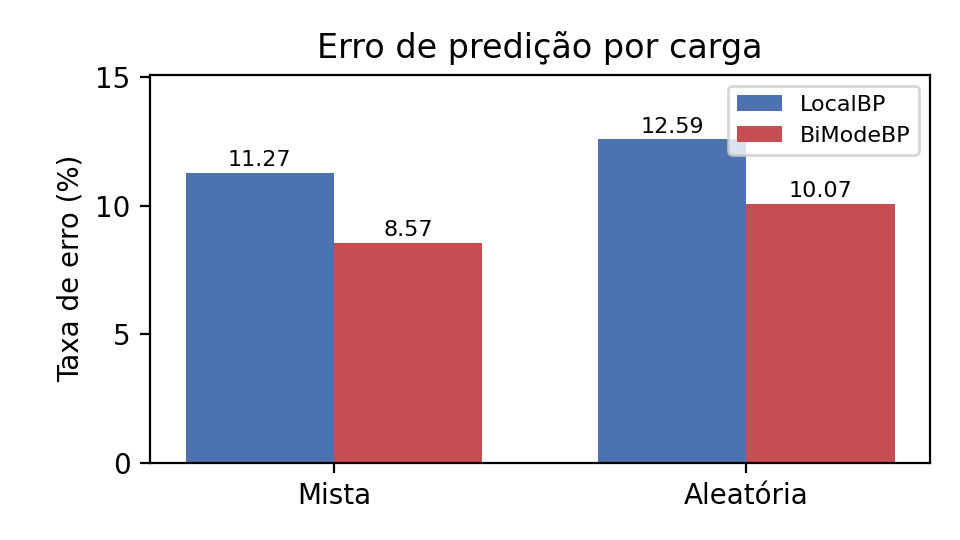
\includegraphics[width=\textwidth]{wl_mispred.png}
  \caption{Taxa de erro por carga e preditor.}
  \label{fig:wlmis}
\end{minipage}\hfill
\begin{minipage}{0.48\textwidth}
  \centering
  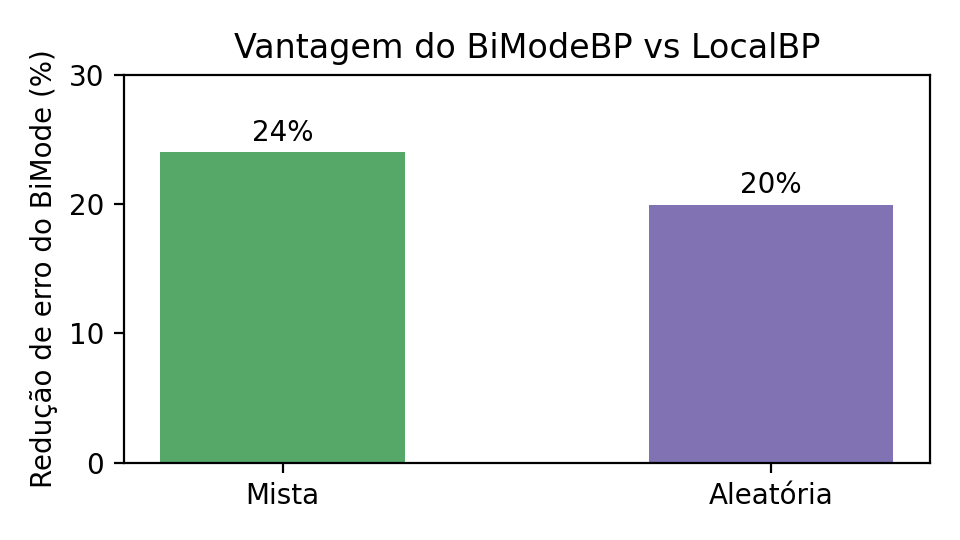
\includegraphics[width=\textwidth]{wl_advantage.png}
  \caption{Vantagem relativa do BiModeBP encolhe na carga aleatória.}
  \label{fig:wladv}
\end{minipage}
\end{figure}

\FloatBarrier

\section{Discussão}

Para esta carga de trabalho, o \textbf{BiModeBP é o preditor mais
adequado}. O motor Monte Carlo é dominado por desvios dependentes de dados
aleatórios e por máquinas de estado com muitos ramos correlacionados (ex.:
``se MP $<$ 150 então farmar; senão se HP do inimigo $>$ 50\% então
atacar''). Essa correlação entre desvios é justamente o que o
histórico global do BiModeBP captura e o LocalBP, restrito ao histórico
por PC, não enxerga. A separação em tabelas ``tomada'' e ``não tomada''
também reduz o \emph{aliasing} destrutivo gerado pela quantidade de pontos
de decisão no laço das 1.000 partidas.

O ganho de desempenho (+3,8\% de IPC), embora consistente, é moderado:
parte dos desvios depende de valores genuinamente aleatórios e é, por
natureza, imprevisível --- nenhum preditor acerta uma moeda justa. O
BiModeBP extrai o máximo da parcela \emph{estruturada} (laços e máquinas
de estado), ao custo de maior complexidade de \emph{hardware}.

\section{Conclusão}

Comparamos LocalBP e BiModeBP sobre um binário RISC-V estático com forte
carga de desvios, simulado no gem5. O preditor global complexo (BiModeBP)
superou o local simples em todas as métricas: taxa de erro de 8,57\% vs.
11,27\%, IPC 3,8\% maior, tempo 4,7\% menor e 38\% menos instruções
descartadas. O resultado confirma a teoria: cargas com desvios
correlacionados --- máquinas de estado e laços de simulação --- se
beneficiam de preditores com histórico global, justificando seu custo de
\emph{hardware}.

O segundo experimento qualifica essa conclusão: ao tornar as decisões
puramente aleatórias, os dois preditores pioram e a vantagem do BiModeBP
cai de 24\% para 20\%. O valor de um preditor sofisticado não é absoluto
--- depende de quanta estrutura a carga oferece. Para este algoritmo, que
mistura forte componente determinística com aleatoriedade, o BiModeBP
ainda compensa, mas a margem é ditada pelo padrão de desvios da carga.

\bibliographystyle{sbc}
\bibliography{referencias}

\end{document}
